\documentclass{article}
\usepackage{graphicx}
\usepackage{hyperref}
\usepackage{color}
\usepackage{marginnote}
\usepackage{mathtools}
\usepackage{amsmath}
\usepackage{amsfonts}
\usepackage{empheq}
\usepackage{listings}

\newcommand{\hilight}[1]{\colorbox{yellow}{#1}}
\newcommand{\boxedeq}[2]{\begin{empheq}[box={\fboxsep=6pt\fbox}]{align}\label{#1}#2\end{empheq}}

\begin{document}

\title{Discretization of an RC Lowpass Filter}
\author{
	Ross Bencina \\
	\texttt{\url{http://www.rossbencina.com}}\\
	\texttt{rossb@audiomulch.com}
}

\date{\today\footnote{An earlier version appeared as a Google document in July 2014. The current version is archived at \url{https://github.com/RossBencina/dsp-notes} and may be revised from time to time. Corrections and bug reports are welcome. }}
	
\maketitle

\section{Introduction}

This note derives a digital version of an
analog RC lowpass filter\footnote{\url{https://en.wikipedia.org/wiki/RC_circuit#Series_circuit}}
 using nodal analysis and trapezoidal integration.
It follows the method used by Andrew Simper in his recent technical notes.\footnote{See Simper's
\href{http://www.cytomic.com/files/dsp/OnePoleLinearLowPass.pdf}{``Direct Numerical Integration of a One Pole Linear Low Pass Filter''} and other technical papers located at
\url{http://www.cytomic.com/technical-papers}.}
The aim is to lay out the mathematical steps that underpin the method, more or less from first principles.
It's a first step towards modelling analog circuits using numerical methods.

Some knowledge of calculus and a little familiarity with linear circuits is assumed (e.g. application of Ohm's Law and Kirchoff's Laws to form nodal equations). Familiarity with digital IIR filters is also assumed (i.e. the idea of a digital filter with state variables and a state update procedure that computes an output sample from an input sample at each time step).

\section{The circuit}

The analog RC lowpass circuit is shown in Figure \ref{fig:RC-lowpass-circuit}.
$R$ is the resistance of the resistor. $C$ is the capacitance of the capacitor.
Our goal is to create a discrete time digital implementation of this circuit.
We want a program that takes voltage $V_{in}$ at each time step and gives us $V_{C}$.

\begin{figure}[here]
	\centering
	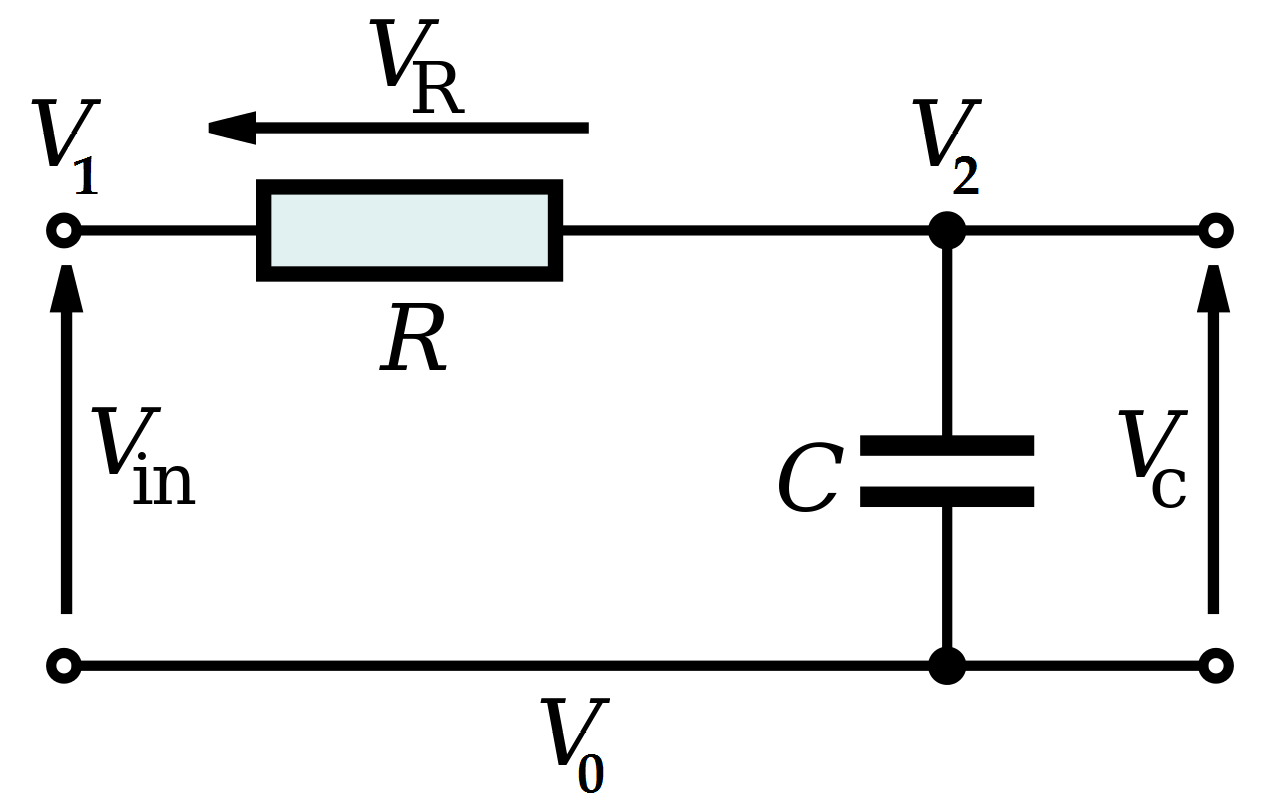
\includegraphics[width=0.5\textwidth]{images/1280px-RC_Series_Filter.png}
	\caption{Analog RC lowpass circuit. 
		Image source: {\href{https://en.wikipedia.org/wiki/File:RC_Series_Filter_(with_V&I_Labels).svg}{Wikipedia}}}
	\label{fig:RC-lowpass-circuit}
\end{figure}


\section{Voltages across the components}

The process of deriving the digital implementation involves solving equations for
the circuit using Ohm's Law and Kirchoff's laws. This process is called nodal analysis.\footnote{\url{http://en.wikipedia.org/wiki/Nodal_analysis}}

We apply the node voltage method\footnote{\url{http://en.wikipedia.org/wiki/Nodal_analysis}} to produce an equation for the voltage across the resistor ($V_R$). The voltage across the capacitor $V_C$ is an unknown that we will solve for later.

Assume that electron current flows in the direction of the arrows.\footnote{For our method to succeed, the direction of the arrows doesn't matter so long as they are kept consistent for the whole calculation. See for example \href{https://www.physicsforums.com/threads/node-voltage-analysis.246884/}{this discussion at physicsforums.com}.}
Applying the formula ($V_{highest} - V_{lowest}$) for the voltage across a component yields $V_R$ as follows:

\begin{align}
V_1 &= V_0 + V_{in}\\
V_2 &= V_0 + V_C\\
V_R &= V_1 - V_2\\
\implies V_R &= (V_0 + V_{in}) - (V_0 + V_C)\\
\label{eqn:V_R}
\implies V_R &= V_{in} - V_C
\end{align}

\section{Current flow for each component}

We need to know the (effective\footnote{Depending on your point of view, current may not flow ``through''
	capacitors. In our model we're going to assume
	\href{https://www.youtube.com/watch?v=ppWBwZS4e7A}{current flows
		through capacitors} and call it $I_C$.}) current flow through each component.

Recall Ohm's Law for a general resistor:

\boxedeq{}{
	I=\frac{V}{R}
}

Using the equation for $V_R$ from above (\ref{eqn:V_R}) gives us the current through the resistor:

\begin{align}
I_R &= \frac{1}{R}V_R\\
\label{eqn:I_R1}
\implies I_R &= \frac{1}{R}(V_{in} - V_C)
\end{align}

The equivalent law for capacitors is:\footnote{\url{https://en.wikipedia.org/wiki/Capacitor#Current.E2.80.93voltage_relation}}

\boxedeq{}{
	I=C\frac{\mathrm{d}V}{\mathrm{d}t}
}

So the current in and out of the capacitor is:

\begin{equation}
\label{eqn:I_C1}
I_C = C\frac{\mathrm{d}}{\mathrm{d}t}V_C
\end{equation}


\section{A differential equation for the circuit \label{sec:diff-eqn}}

Kirchoff's current law (KCL)\footnote{\url{https://en.wikipedia.org/wiki/Kirchhoff's_circuit_laws}}
tells us that the sum of currents into a node
equals the sum of currents out of the node. For node $V_2$ this yields

\begin{equation}
I_R = I_C
\end{equation}

Substituting the expressions above for $I_R$ (\ref{eqn:I_R1}) and $I_C$ (\ref{eqn:I_C1}):

\begin{equation}
\frac{1}{R}(V_{in} - V_C) = C\frac{\mathrm{d}}{\mathrm{d}t}V_C
\label{eqn:nodal-equation}
\end{equation}

Our goal is to produce a numerical solution to equation \ref{eqn:nodal-equation} for $V_C$ (the circuit output) given $V_{in}$ (the
circuit input) at each time step. To do this we discretize
(approximate) the capacitor using a linear approximation and then
expand the KCL equations using the discretized expression for $I_C$.

\section{Aside: current-voltage relation for a capacitor}

This section is a bit of an aside. We're going to compute a result
that's needed in the next section. It relates capacitor voltage and
current. If you're happy to take the relation as given you can skip this
section. In summary, we will show that equation \ref{eqn:I_C1}:

\begin{equation}
\notag
I_C = C\frac{\mathrm{d}}{\mathrm{d}t}V_C
\end{equation}

implies:

\begin{equation}
\notag
	V_C(t) = \frac{1}{C}\int_{t_0}^{t} \! I_C(\tau) \, \mathrm{d}\tau + V_C(t_0)
\end{equation}

This is a well known relation that expresses voltage across a capacitor
at time $t$ as the sum of the voltage at an earlier time $t_0$, plus an
integration of $I_C$ (current) over the time range $t_0$ to $t$. In the
next section we'll use the relation to construct a discrete time
time-step update equation for the voltage across a capacitor.

To derive the current voltage relation, recall equation \ref{eqn:I_C1}
for current flow in and out of a capacitor:

\begin{align}
\notag
I_C &= C\frac{\mathrm{d}}{\mathrm{d}t}V_C, &\text{(equation \ref{eqn:I_C1})}
\intertext{
rearranging and making time an explicit parameter \tau:
}
\notag
\frac{\mathrm{d}}{\mathrm{d}t}V_C(\tau) &= \frac{1}{C}I_C(\tau) &\hspace{.25\textwidth}
\\
\intertext{
Integrating both sides from $t_0$ to $t$:\footnotemark
}
\notag
\int_{t_0}^{t} \! \frac{\mathrm{d}}{\mathrm{d}t}V_C(\tau) \, \mathrm{d}\tau
&=
\frac{1}{C}\int_{t_0}^{t} \! I_C(\tau) \, \mathrm{d}\tau
\\
\notag
\left[V_C(\tau)\right]_{t_0}^{t}
&=
\frac{1}{C}\int_{t_0}^{t} \! I_C(\tau) \, \mathrm{d}\tau
\\
\notag
V_C(t) - V_C(t_0)
&=
\frac{1}{C}\int_{t_0}^{t} \! I_C(\tau) \, \mathrm{d}\tau
\\
\label{eqn:V_C_t}
V_C(t)
&=
V_C(t_0) + \frac{1}{C}\int_{t_0}^{t} \! I_C(\tau) \, \mathrm{d}\tau
\end{align}
\footnotetext{
	See: \url{http://www.site.uottawa.ca/mathasatool/01unit/12topic/focus/voltage_current/p09.htm}
}

Notice that given two times $t_0$ and $t$, 
equation \ref{eqn:V_C_t} gives us a way to compute $V_C(t)$ as a function of
$V_C(t_0)$ and a definite integral over $I_C$ from time $t_0$ to
time $t$.


\section{Discretizing a capacitor using the trapezoidal rule}

In the previous section we derived a general time-domain relation (equation \ref{eqn:V_C_t}) for
the capacitor currents and voltages at times $t_0$ and $t$.
We'll use the general relation to derive a time-step update
rule (difference equations) for our uniformly sampled (digital) system.
The update rule takes us from the previous time step to the current time
step.

Let $sr$ be the sampling rate in samples per second.

Let $T$ be the sampling period: $T = 1/sr$

Let $t$ be the time of the current time step

Take $t_0$ to be the time of the previous time step, that is $t_0 = t - T$

Discretizing the current/voltage relation for time $t$, first substitute
$t$ and $T$ into equation \ref{eqn:V_C_t} from the previous section:

\begin{align}
V_C(t) &= V_C(t_0) + \frac{1}{C}\int_{t_0}^{t} \! I_C(\tau) \, \mathrm{d}\tau &\text{(from equation \ref{eqn:V_C_t})}\\
\label{eqn:V_C_t_a}
       &= V_C(t-T) + \frac{1}{C}\int_{t_0}^{t} \! I_C(\tau) \, \mathrm{d}\tau &\text{($t_0 = t - T$)}
\intertext{
Now we apply the trapezoidal rule to discretize the integral. The trapezoidal rule states:\footnotemark
}
\label{eqn:trap-rule}
\int_a^b \! f(x) \, \mathrm{d}x &\approx (b-a)\frac{(f(a) + f(b))}{2} \\
\intertext{
	We will use the trapezoidal rule to approximate the following integral:
}
\frac{1}{C}\int_{t_0}^{t} \! I_C(\tau) \, \mathrm{d}\tau &\approx \, ? \\
\intertext{
	Making the following substitutions to the trapazoidal rule (\ref{eqn:trap-rule}):
}
\notag f(x)&: I_C(x) \\
\notag a&: (t-T), \\
\notag b&: (t), \\
\notag (b-a) &= t-(t-T) = t-t+T \\
\notag \implies (b-a) &: T\\
\intertext{
	yeilds:
}
\frac{1}{C}\int_{t_0}^{t} \! I_C(\tau) \, \mathrm{d}\tau &\approx \frac{T}{2C} (I_C(t-T) + I_C(t))
\intertext{
	Substituting this approximation into equation \ref{eqn:V_C_t_a} gives an expression for $V_C(t)$ in terms of voltages and currents at the current and previous time steps:
}
\label{eqn:trap-V_C}
V_C(t) &\approx V_C(t-T) + \frac{T}{2C} (I_C(t-T) + I_C(t))
\end {align}
\footnotetext{
	Trapezoidal rule: 
	\url{https://en.wikipedia.org/wiki/Trapezoidal_rule}
	\url{http://www.mathwords.com/t/trapezoid_rule.htm}
}

The trapezoidal rule is an approximation, but we will treat equation \ref{eqn:trap-V_C} as an equivalent expression for $V_C$ from here on.

Let's switch our notation to the discrete time domain and to something more closely resembling computer code. We'll notate multiplication with ``$.$''.
Take $n \in \mathbb{Z}$ as the current time step and $n-1$ as the previous time step.
Switch notation as follows:

\begin{align*}
V_C(t) &\to vc[n] \\
V_C(t-T) &\to vc[n-1] \\
I_C(t) &\to ic[n] \\
I_C(t-T) &\to ic[n-1] \\
\end{align*}

Rewriting the trapezoidally integrated equation for $V_C$ (\ref{eqn:trap-V_C}):

\begin{equation}
\label{eqn:trap-V_C-discrete}
vc[n] = vc[n-1] + T/(2C) . ( ic[n-1] + ic[n] )
\end{equation}

Later, when applying KCL we will want an expression for $ic[n]$. So,
	solve equation \ref{eqn:trap-V_C-discrete} for $ic[n]$:

\begin{align}
\implies &vc[n] - vc[n-1] = T/(2C) . ic[n-1] + T/(2C) . ic[n] \notag\\
\implies &vc[n] - vc[n-1] - T/(2C) . ic[n-1] = T/(2C) . ic[n] \notag\\
\implies &ic[n] = (2C)/T . (vc[n] - vc[n-1]) - ic[n-1]
\end{align}

Letting $gc = (2C)/T$:

\begin{equation}
ic[n] = gc . vc[n] + (- gc . vc[n-1] - ic[n-1])
\end{equation}

Following a convention used by QUCS using ``iceq'':\footnote{
	See e.g. \href{http://qucs.sourceforge.net/tech/node26.html#SECTION00731000000000000000}{equations 6.60 and 6.63 in the QUCS documentation}}

Let

\begin{eqnarray} \begin{array}{l}
iceq[n-1] = - gc . vc[n-1] - ic[n-1]\\
ic[n] = gc . vc[n] + iceq[n-1].
\end{array} \end{eqnarray}

Or equivalently:

\begin{eqnarray} \begin{array}{l}
\label{eqn:ic_n}
ic[n] = gc . vc[n] + iceq[n-1]\\
iceq[n] = - gc . vc[n] - ic[n].
\end{array} \end{eqnarray}

We can further simplify $iceq$ by substituting for $ic[n]$

\begin{align}
&iceq[n] = - gc . vc[n] - ic[n] \notag\\
\implies &iceq[n] = - gc . vc[n] - (gc . vc[n] + iceq[n-1])\notag\\
\implies &iceq[n] = -2 . gc . vc[n] - iceq[n-1].
\end{align}


\section{Solving the KCL equation(s) using the linear equivalent capacitor current}

Remember the differential equation from section \ref{sec:diff-eqn}?
We're ready to solve the equivalent linear equation. Instead of 
$I_C = C\frac{\mathrm{d}}{\mathrm{d}t}V_C$
we'll be using the linear approximation $ic[n]$ derived in the previous section (\ref{eqn:ic_n}).

Recall,

\begin{equation}
\begin{aligned}
		   I_R &= (1/R) (V_{in} - V_C)	 	&\text{(current through the resistor)} \\
\to	     ir[n] &= (1/R) . (vin[n] - vc[n])\\
\\
	      	gc &= (2C)/T \hspace{.1\textwidth}& \\
	      	iceq[n] &= -2 . gc . vc[n] - iceq[n-1] \\
	     ic[n] &= gc . vc[n] + iceq[n-1]    &\text{(current ``through'' the capacitor)}
\end{aligned}
\end{equation}

Equating current in and current out at our node of interest:

\begin{equation}
\begin{aligned}
                   I_R &= I_C	 	&\text{(KCL: currents in and out of a node are equal)} \\
\to                 ir[n] &= ic[n]	\hspace{.1\textwidth}& \\
\implies (1/R) . (vin[n] - vc[n]) &= gc . vc[n] + iceq[n-1] &
\end{aligned}
\end{equation}

\textit{
(In general we would have a set of simultaneous equations to
	solve, one equation for each node. However, in this case we have only
	one node.)
}


Now the final step. Given our input $vin[n]$ we want to compute $vc[n]$.

Solving the previous equation for $vc[n]$:

\begin{equation}
\begin{aligned}
     (1/R) . (vin[n] - vc[n]) &= gc . vc[n] + iceq[n-1] \\
\implies (1/R) . vin[n] - (1/R) . vc[n] - gc . vc[n] - iceq[n-1] &= 0 \\
\implies (1/R) . vin[n] - iceq[n-1] 	&= (1/R) . vc[n] + gc . vc[n] \\
\implies vin[n] - R . iceq[n-1] 		&= vc[n] + R . gc . vc[n]			&\text{(times R)} \\
                            &= vc[n] . (1 + R.gc) \\
\implies                   vc[n] 	&= (vin[n] - R . iceq[n-1]) / (1 + R.gc)
\end{aligned}
\end{equation}

So our final equations are:

\begin{align}
 gc = (2C)/T\\
 vc[n] &= (vin[n] - R . iceq[n-1]) / (1 + R.gc)\\
 iceq[n] &= (- 2.gc.vc[n] - iceq[n-1])
\end{align}

or, letting $gr = 1/R$

\begin{align}
vc[n] &= (gr . vin[n] - iceq[n-1]) / (gr + gc)\\
iceq[n] &= (- 2.gc.vc[n] - iceq[n-1])
\end{align}

Or equivalently:

\begin{align}
vc[n] &= (gr . vin[n] + iceq[n-1]) / (gr + gc)\\
iceq[n] &= 2.gc*vc[n] - iceq[n-1]
\end{align}

Andrew Simper suggests setting $gc=1$, $gr=g$

\begin{align}
vc[n] &= (g . vin[n] + iceq[n-1]) / (1 + g)\\
iceq[n] &= 2.vc[n] - iceq[n-1]
\end{align}

In pseudo-code:

\begin{lstlisting}
init:
    iceq = 0

step (input: vin, output: vc):
    vc = (g * vin + iceq) / (1 + g)
    iceq = 2 * vc - iceq
\end{lstlisting}



\section{Acknowledgements}

The method described here is an interpretation of Andrew Simper's worked example,\footnote{\url{http://www.cytomic.com/files/dsp/OnePoleLinearLowPass.pdf}} 
and his related papers.\footnote{\url{http://www.cytomic.com/technical-papers}} 
Thanks to Andrew and other members of the
\#musicdsp IRC channel for their very kind assistance in guiding me
through this.

\end{document}